\subsubsection{UC\theuccount-GP - Rimozione utente dal sistema}
		\begin{figure}[H]
			\centering
				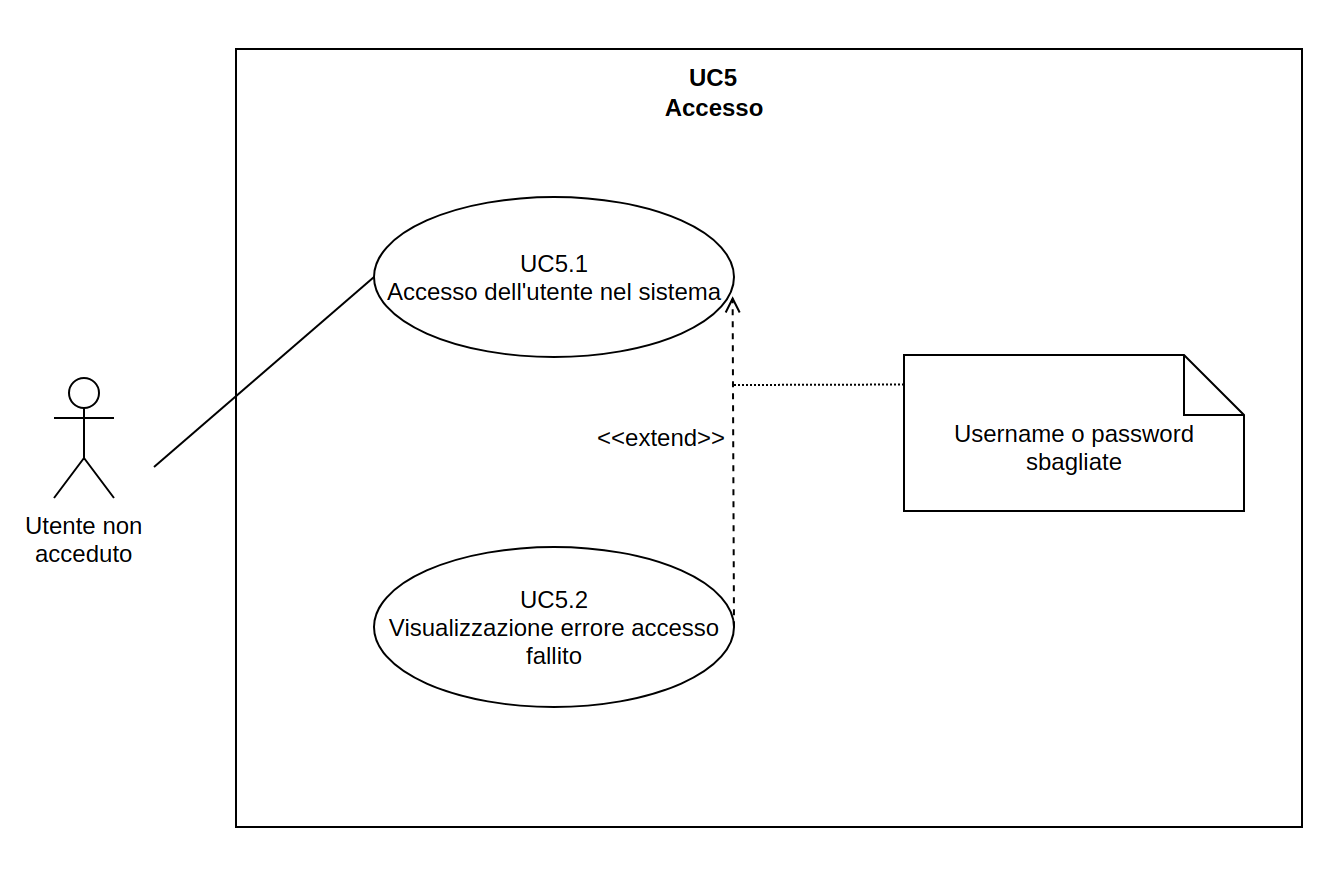
\includegraphics[width=\columnwidth]{img/UC5.png}\\
			\caption{UC\theuccount-GP - Rimozione utente dal sistema}
		\end{figure}
	\begin{itemize}
		\item \textbf{Codice}: UC\theuccount-GP.
		\item \textbf{Titolo}: Rimozione utente dal sistema.
		\item \textbf{Attori primari}: utente acceduto.
		\item \textbf{Descrizione}: l'utente rimuove l'utente desiderato dal sistema.
		\item \textbf{Precondizione}: un utente già presente deve essere rimosso dal sistema.
		\item \textbf{Postcondizione}: un utente viene rimosso dal sistema.
		\item \textbf{Scenario Principale}:
		\begin{enumerate}
			\item Utente acceduto procede alla rimozione di un utente.
		\end{enumerate}
\end{itemize}

	\paragraph{UC\theuccount.1-GP - Rimozione avvenuta con successo}
		\begin{figure}[H]
			\centering
			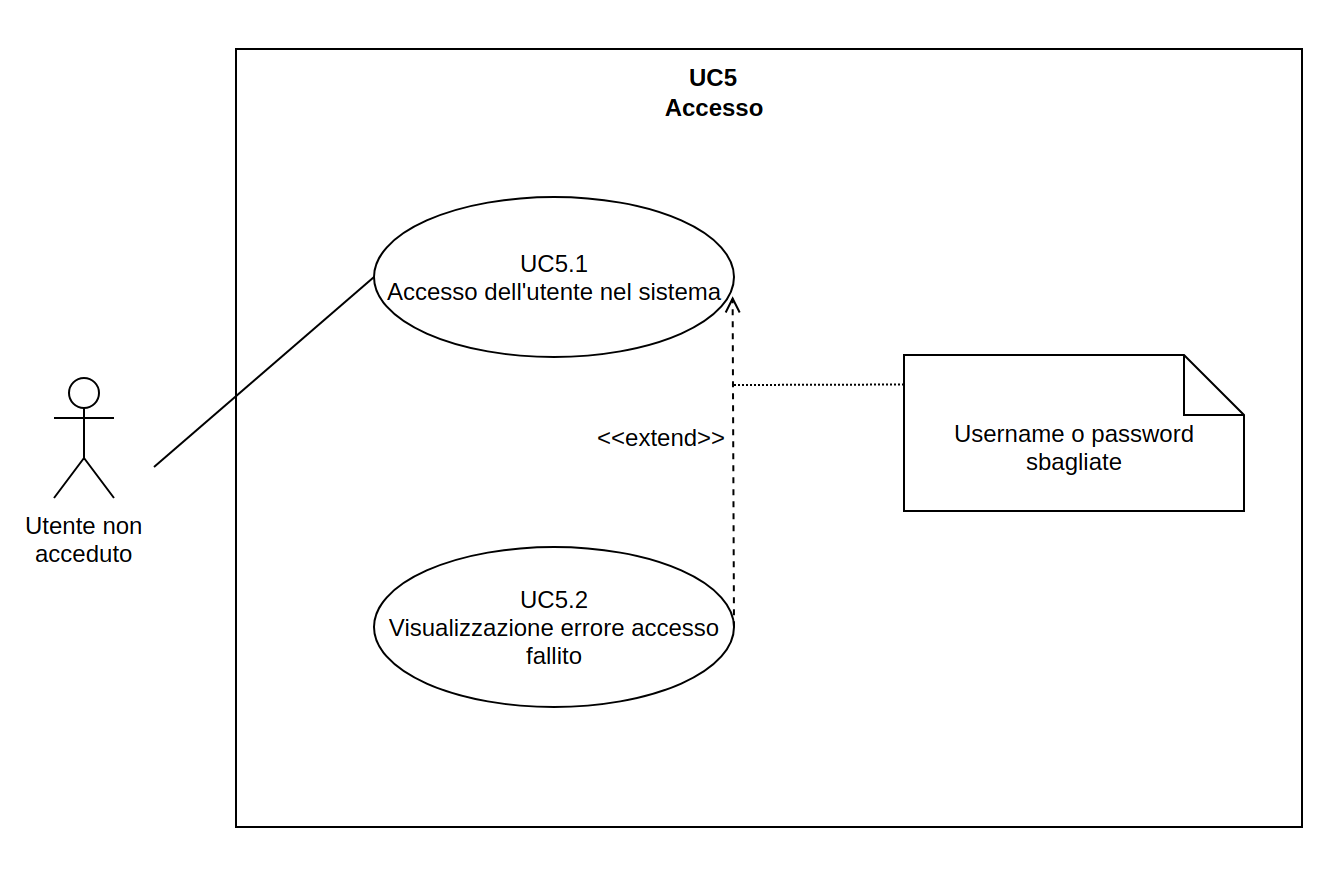
\includegraphics[width=\columnwidth]{img/UC5.png}\\
			\caption{UC\theuccount.1-GP - Rimozione avvenuta con successo}
		\end{figure}
		\begin{itemize}
			\item \textbf{Codice}: UC\theuccount.1-GP.
			\item \textbf{Titolo}: rimozione avvenuta con successo.
			\item \textbf{Attori primari}: utente acceduto.
			\item \textbf{Descrizione}: il contatto Email o Telegram desiderato è presente nel sistema,
			per cui la rimozione avviene con successo.
			\item \textbf{Precondizione}: un utente già presente deve essere rimosso dal sistema.
			\item \textbf{Postcondizione}: un utente con il contatto Email o Telegram inserito viene rimosso dal sistema.
			\item \textbf{Scenario Principale}:
			\begin{enumerate}
				\item Un utente viene rimosso.
			\end{enumerate}
			\item \textbf{Estensioni}:
			\begin{itemize}
				\item Errore contatto non presente nel sistema[UC14.2-GP].
			\end{itemize}
		\end{itemize}

			\subparagraph{UC\theuccount.1.1-GP - Inserimento contatto Email}
				\begin{figure}[H]
					\centering
					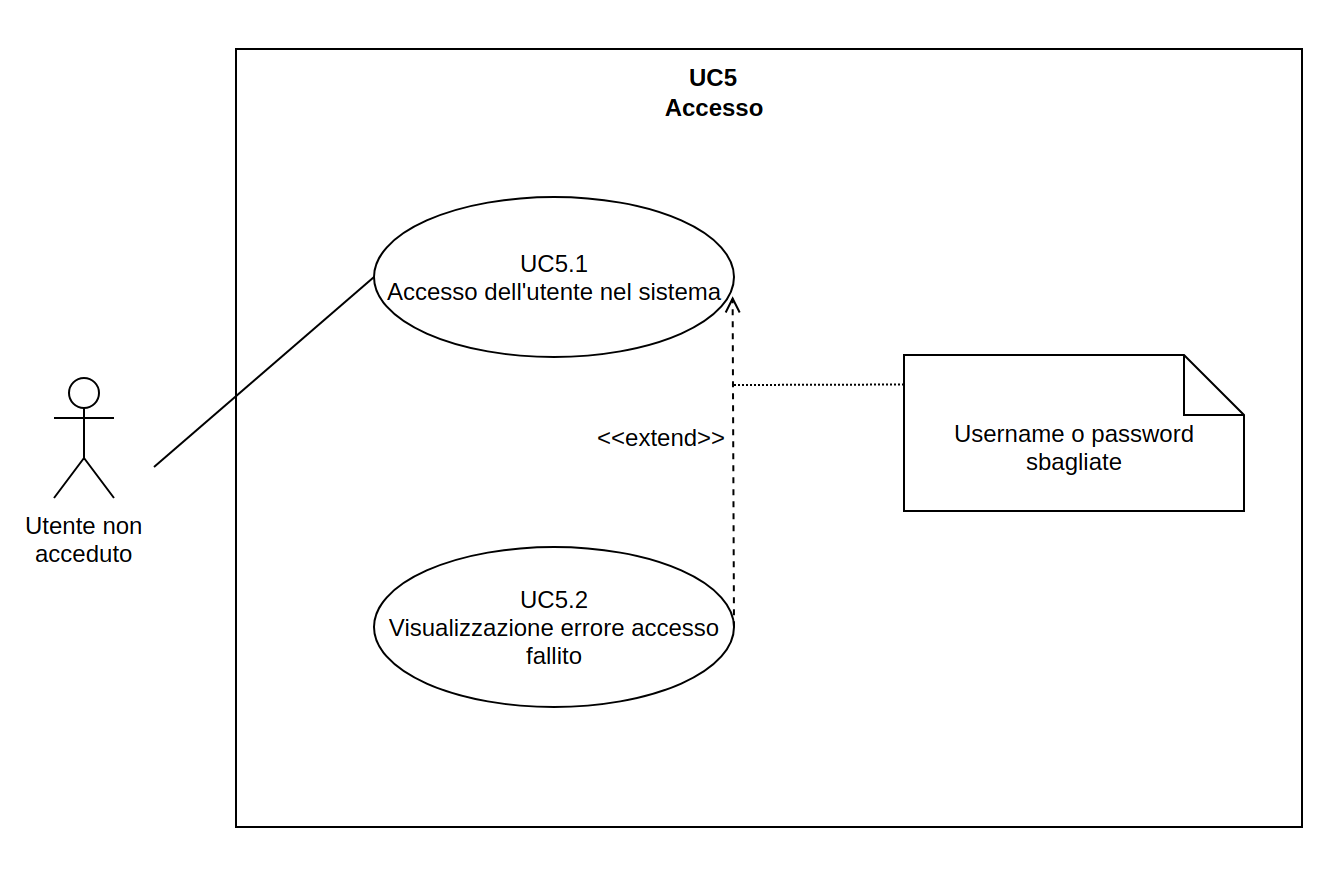
\includegraphics[width=\columnwidth]{img/UC5.png}\\
					\caption{UC\theuccount.1.1-GP - Inserimento contatto Email}
				\end{figure}
				\begin{itemize}
					\item \textbf{Codice}: UC\theuccount.1.1-GP.
					\item \textbf{Titolo}: inserimento contatto Email.
					\item \textbf{Attori primari}: utente acceduto.
					\item \textbf{Descrizione}: l'utente ha aggiunto il contatto Email relativo all'utente che vuole rimuovere.
					\item \textbf{Precondizione}: un utente già presente deve essere rimosso dal sistema.
					\item \textbf{Postcondizione}: il contatto Email è stato inserito.
					\item \textbf{Scenario Principale}:
					\begin{enumerate}
						\item Utente acceduto procede all'inserimento del contatto Email del utente da rimuovere.
					\end{enumerate}
				\end{itemize}

				\subparagraph{UC\theuccount.1.2-GP - Inserimento contatto Telegram}
					\begin{figure}[H]
						\centering
						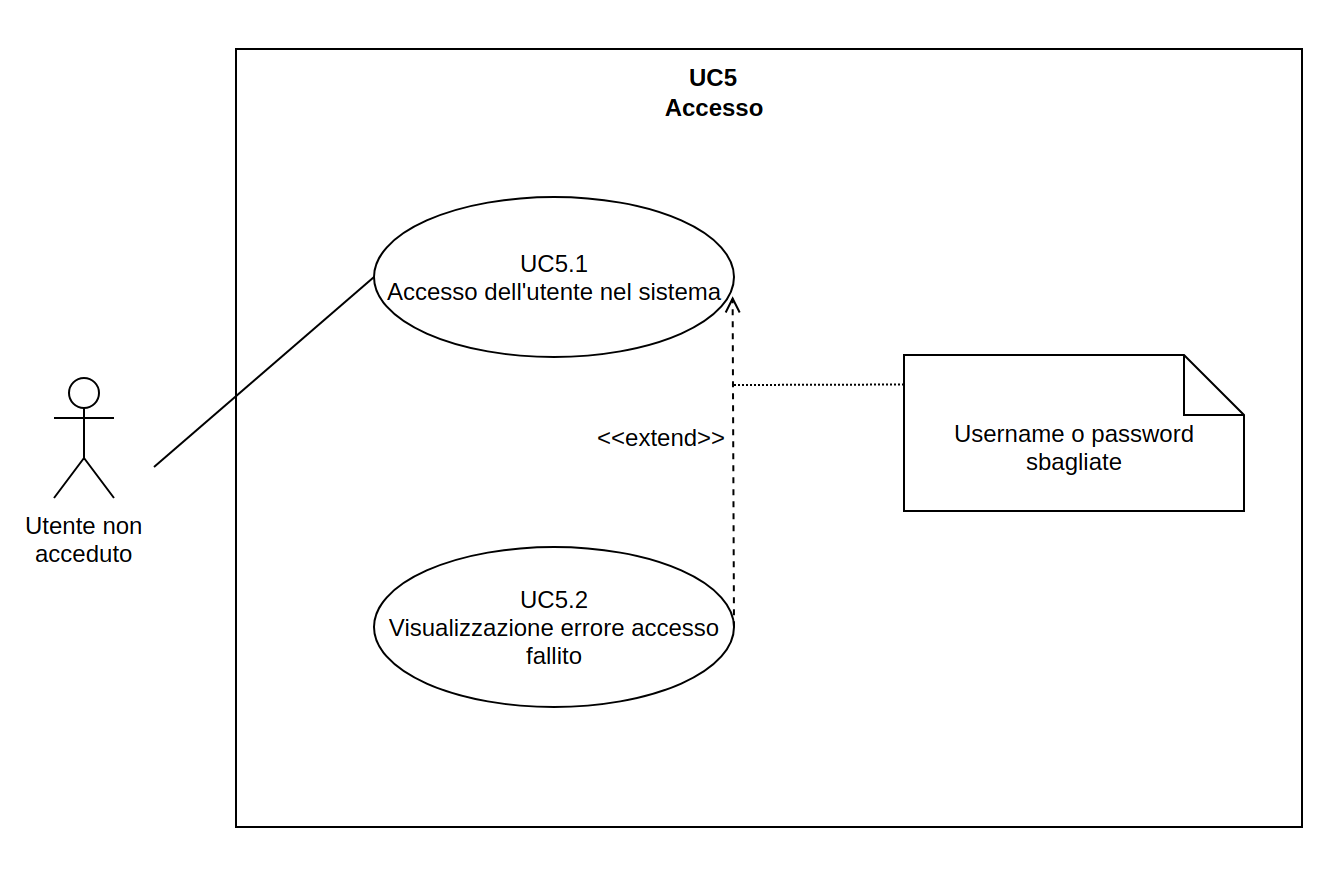
\includegraphics[width=\columnwidth]{img/UC5.png}\\
						\caption{UC\theuccount.1.2-GP - Inserimento contatto Telegram}
					\end{figure}
					\begin{itemize}
						\item \textbf{Codice}: UC\theuccount.1.2-GP.
						\item \textbf{Titolo}: inserimento contatto Telegram.
						\item \textbf{Attori primari}: utente acceduto.
						\item \textbf{Descrizione}: l'utente ha aggiunto il contatto Telegram relativo all'utente che vuole rimuovere.
						\item \textbf{Precondizione}: un utente già presente deve essere rimosso dal sistema.
						\item \textbf{Postcondizione}: il contatto Telegram è stato inserito.
						\item \textbf{Scenario Principale}:
						\begin{enumerate}
							\item Utente acceduto procede all'inserimento del contatto Telegram del utente da rimuovere.
						\end{enumerate}
					\end{itemize}

				\paragraph{UC\theuccount.2-GP - Errore contatto non presente nel sistema}
						\begin{figure}[H]
							\centering
							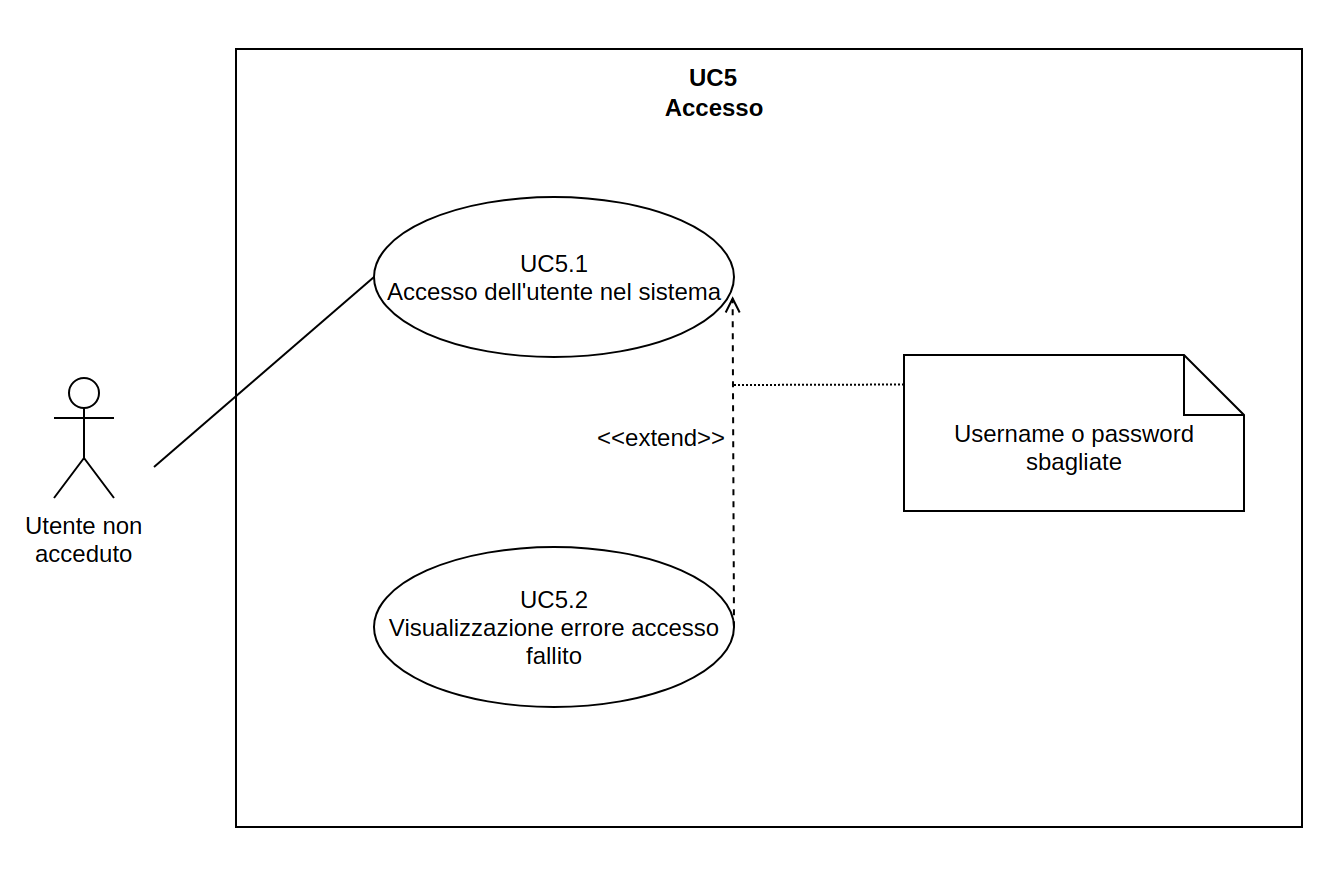
\includegraphics[width=\columnwidth]{img/UC5.png}\\
							\caption{UC\theuccount.2-GP - Errore contatto non presente nel sistema}
						\end{figure}
						\begin{itemize}
							\item \textbf{Codice}: UC\theuccount.2-GP.
							\item \textbf{Titolo}: errore contatto non presente nel sistema.
							\item \textbf{Attori primari}: utente acceduto.
							\item \textbf{Descrizione}: l’utente viene avvisato che il contatto inserito non è presente nel sistema.
							\item \textbf{Precondizione}: un utente già presente deve essere rimosso dal sistema.
							\item \textbf{Postcondizione}: il sistema comunica all’utilizzatore l’errore e nessuno user viene rimosso.
							\item \textbf{Scenario Principale}:
							\begin{enumerate}
								\item Un utente non viene rimosso perchè non presente nel sistema.
							\end{enumerate}
						\end{itemize}